\documentclass[12pt,a4paper]{ctexart}

\usepackage[UTF8]{ctex}
\usepackage{geometry}
\usepackage{graphicx}
\usepackage{xcolor}
\usepackage{tikz}
\usepackage{fontspec}
\usepackage{setspace}
\usepackage{enumitem}
\usepackage{booktabs}
\usepackage{array}
\usepackage{longtable}
\usepackage{hyperref}
\usepackage{fancyhdr}
\usepackage{titlesec}
\usepackage{multicol}
\usepackage{xurl}
\usepackage{tocloft}

\renewcommand{\cfttoctitlefont}{\hfill\bfseries\Large}
\renewcommand{\cftaftertoctitle}{\hfill}
\geometry{left=2.5cm,right=2.5cm,top=2.5cm,bottom=2.5cm}

\definecolor{black}{RGB}{0,0,0}
\definecolor{mainblue}{RGB}{0,82,147}
\definecolor{accentgold}{RGB}{180,140,60}
\definecolor{lightgray}{RGB}{245,245,245}
\definecolor{darkgray}{RGB}{80,80,80}
\definecolor{mainred}{RGB}{230,1,45}

\hypersetup{
    colorlinks=true,
    linkcolor=black,
    urlcolor=mainblue,
    citecolor=mainblue,
    pdfborder={0 0 0}
}

\pagestyle{fancy}
\fancyhf{}
\fancyhead[L]{\small\color{darkgray}\textbf{量子行业每周新闻洞察}}
\fancyhead[R]{\small\color{darkgray}\textbf{总第187期}}
\fancyfoot[C]{\thepage}
\renewcommand{\headrulewidth}{0.4pt}
\renewcommand{\footrulewidth}{0pt}

\titleformat{\section}
    {\Large\bfseries\color{mainred}}
    {\thesection、}{0em}{}
\titleformat{\subsection}
    {\large\bfseries\color{mainred}}
    {\thesubsection、}{0em}{}

\newcolumntype{L}[1]{>{\raggedright\arraybackslash}p{#1}}
\newcolumntype{C}[1]{>{\centering\arraybackslash}p{#1}}

\begin{document}

% ==================== 封面 ====================
\begin{titlepage}
\begin{tikzpicture}[remember picture,overlay]
    \fill[mainred] ([yshift=-0.5cm]current page.north west) rectangle ([yshift=-1.2cm]current page.north east);
    \fill[mainred] ([yshift=1.2cm]current page.south west) rectangle ([yshift=0.5cm]current page.south east);
\end{tikzpicture}

\vspace*{4cm}

\begin{center}
    {\fontsize{44}{52}\selectfont\bfseries\color{black} \textbf{量子行业每周新闻洞察}}

    \vspace{0.8cm}

    {\fontsize{16}{22}\selectfont\color{darkgray} 2026.07.04 — 2026.07.10 }
    {\fontsize{16}{22}\selectfont\color{darkgray} \textbf{WEEKLY NEWS}}

    \vspace{1.5cm}

    {\fontsize{20}{26}\selectfont\color{mainred}\textbf{（总第\textbf{ 187 }期）}}

    \vspace{4cm}

    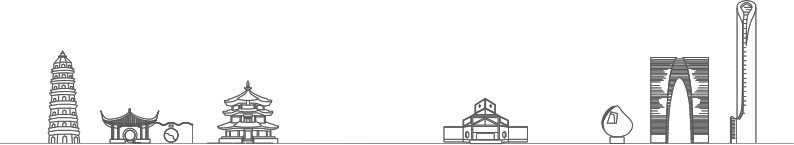
\includegraphics[width=\textwidth]{Cover_Suzhou.png}

    \vfill

    {\fontsize{12}{16}\selectfont\color{darkgray} 量子科技长三角产业创新中心\\编制：战略情报与成果专利室、产业发展部（理事会办公室）}
\end{center}
\end{titlepage}

% ==================== 目录 ====================
\pagenumbering{roman}
\newpage
\tableofcontents

\newpage

% ==================== 摘要 ====================
\pagenumbering{arabic}
\setcounter{page}{1}
\begin{center}
{\Large\bfseries\color{mainred} 摘\hspace{2em}要}
\end{center}
\addcontentsline{toc}{section}{摘要}


\textbf{ 宏观态势：}

全球量子科技竞争进入战略落地新阶段。美国通过白宫峰会强化顶层设计，联邦机构量子计算试点率快速攀升，凸显政府需求的牵引作用。欧洲与日本则通过Q-Neko等跨国项目，聚焦构建量子与高性能计算融合的生态系统。与此同时，Xthings启动后量子密码战略，表明在智能环境等场景中，应对量子威胁的“加密敏捷”能力正从概念走向基础设施层面的部署，安全考量与产业应用的结合日益紧密。


\textbf{ 科技前沿：}

基础研究持续向量子世界的精度极限与实用边界挺进。一方面，科学家正深挖材料物性，联合项目推动量子材料发展，首次在量子计算机上实现聚变材料计算。另一方面，对测量本质的认知被刷新，如揭示电子位置与时间演化无法同时精确测量。技术路线上，室温液晶可调谐激光器和金属氢化物激光冷却等突破，展示了向更易用、更常规条件推进的努力，而利用机械振动提升容错能力则为系统鲁棒性提供了新思路。


\textbf{ 产品动态：}

量子计算硬件与安全方案正加快进入实际应用场景。IQM的量子计算机被LUMI AI工厂选用，标志着高性能量子算力开始融入经典超算生态，直接服务于人工智能等前沿科研。工业端，三星借力量子计算与AI追赶芯片制造先进制程，揭示了其在高精尖产业中的潜力。同时，后量子安全平台与英特尔处理器的兼容，以及对芯片表面进行高精度测绘的离子阱技术，反映出量子产品正向兼容现有IT架构、服务于具体工业测量的务实方向演进。


\textbf{ 企业资讯：}

产业生态的全球协作与纵深拓展态势明显。量子计算公司通过跨国合作加速区域布局，如Pasqal推进韩国工业落地、Archer评估在澳本土部署。产业链上下游的捆绑更为紧密，SEALSQ与格芯旨在共建可信半导体生态，TOPPAN与东大设立量子点创新实验室。此外，行业对人才与专业经验的渴求突出，退役将领加入后量子密码公司顾问委员会。量子技术也开始渗透至能源管理等非传统计算领域，应用边界持续拓宽。


\textbf{ 资本运作：}

资本正以更大规模、更精准的方向涌入量子科技赛道。中性原子路线获3亿美元级巨额融资，玻色量子启动科创板上市，标志着技术成熟度正获得资本市场重量级认可。资本布局趋于完整，既有关注基础量子计算芯片制造能力的前沿项目，也有押注软件、AI优化和量子安全等关键配套环节。尤其值得关注的是，通过收购整合补强技术图谱成为趋势，如BTQ收购QPerfect、IQM收购工业软件资产，显示行业正通过并购加速全栈能力构建。




\textbf{ 专利动态：}

本周专利动态涵盖低温环境系统、超导量子测控技术、量子软件与算法、量子算力网共4个板块、21条专利。




% ==================== 会议列表 ====================
{
    \newpage
    \section*{ 7月量子科技行业国内、国际会议}
    \addcontentsline{toc}{section}{ 7月量子科技行业国内、国际会议}
    \scriptsize
    \begin{longtable}{C{0.8cm}L{2.5cm}L{3cm}L{7cm}}
        \toprule[1.5pt]
        \textbf{序号} & \textbf{日期} & \textbf{地点} & \textbf{会议名称} \\
        \midrule
        \endfirsthead
        \toprule
        \textbf{序号} & \textbf{日期} & \textbf{地点} & \textbf{会议名称} \\
        \midrule
        \endhead
        \bottomrule
        \endfoot
        
        1 & 7月1日-3日 & 奥尔堡, 丹麦 & IEEE量子控制、计算与学习国际会议（IEEE qCCL 2026） \\
        \midrule[0.05pt]
        
        2 & 7月1日-3日 & 首尔, 韩国 & 2026量子信息会议（CQI 2026） \\
        \midrule[0.05pt]
        
        3 & 7月1日-3日 & 爱丁堡, 英国 & 2026青年量子研究者暑期学校 \\
        \midrule[0.05pt]
        
        4 & 7月2日-4日 & 首尔, 韩国 & Quantum Korea 2026 \\
        \midrule[0.05pt]
        
        5 & 7月6日-8日 & 海尔布隆, 德国 & 自然科学容错量子计算研讨会（FTQC4NSc） \\
        \midrule[0.05pt]
        
        6 & 7月6日-10日 & 那不勒斯, 意大利 & 第12届单光子研讨会（SPW 2026） \\
        \midrule[0.05pt]
        
        7 & 7月7日-10日 & 加尔各答, 印度 & 2026年IEEE量子计算国际研讨会：电路、系统、自动化与应用（QC-CSAA） \\
        \midrule[0.05pt]
        
        8 & 7月12日-17日 & 马斯特里赫特, 荷兰 & 量子传感与计量学（QSM） \\
        \midrule[0.05pt]
        
        9 & 7月13日-17日 & 代尔夫特, 荷兰 & 第7届自旋量子信息处理会议（Spin Qubit 7） \\
        \midrule[0.05pt]
        
        10 & 7月13日-17日 & 悉尼, 澳大利亚 & IEEE量子软件国际会议（QSW 2026） \\
        \midrule[0.05pt]
        
        11 & 7月16日-18日 & 波尔图, 葡萄牙 & 量子信息、计算、通信与模拟国际会议（QUANTICS 2026） \\
        \midrule[0.05pt]
        
        12 & 7月19日-23日 & 博尔德, 美国 & 有限温度非平衡超流体系统研讨会（FINESS 2026） \\
        \midrule[0.05pt]
        
        13 & 7月20日-24日 & 埃朗根, 德国 & 第30届中欧量子光学研讨会（CEWQO 2026） \\
        \midrule[0.05pt]
        
        14 & 7月22日-23日 & 芝加哥, 美国 & 全球量子论坛（GQF 2026） \\
        \midrule[0.05pt]
        
        15 & 7月25日-26日 & 伊斯顿, 美国 & 量子科学研讨会（Gordon Research Seminar） \\
        \midrule[0.05pt]
        
        16 & 7月26日-31日 & 伊斯顿, 美国 & 多体量子系统：量子计算、模拟、传感与新兴平台（Gordon Research Conference） \\
        \midrule[0.05pt]
        
        17 & 7月26日-8月1日 & 布拉格, 捷克共和国 & 量子与介观热力学前沿2026（FQMT'26） \\
        \midrule[0.05pt]
        
        18 & 7月27日-31日 & 科莫湖, 意大利 & 超快量子光学新前沿暑期学校 \\
        \midrule[0.05pt]
        
        19 & 7月27日-31日 & 艾哈迈达巴德及线上, 印度 & 自由空间量子通信短课程 \\
        \midrule[0.05pt]
        
    \end{longtable}
}




% ==================== 宏观态势 ====================
\newpage
\section{宏观态势}
\vspace{-0.5em}
\noindent\rule{\linewidth}{1.5pt}

\subsection{ 美国白宫已于日前举办“白宫量子创新峰会”，聚焦量子科技领域的创新与发展 }

2026年07月09日消息，美国白宫已于7月7日举办“白宫量子创新峰会”，旨在汇聚产业界力量，聚焦量子信息科学与技术的创新发展。白宫科技政策办公室主任和国家量子协调办公室主任等在峰会上发表了主旨演讲，介绍了特朗普政府在量子议程及研发方面的最新进展。此外，来自美国商务部、国防部、能源部、国家科学基金会等政府机构的多位负责人参与了讨论，并分享了各自部门在量子创新领域的承诺落实进展。

\noindent\textbf{报道链接：}\url{https://www.nextgov.com/emerging-tech/2026/07/white-house-host-quantum-tech-summit-industry-tuesday/414608/}

\subsection{ 欧日15家合作伙伴参与，Q-Neko项目旨在建设量子加速高性能计算生态 }

2026年07月08日消息，由芬兰CSC – IT Center for Science协调的Q-Neko项目旨在帮助欧洲与日本在量子加速高性能计算（HPC+QC）领域建立强大的生态。该项目依托现有欧日合作基础，致力于开发通用方法、基准和标准，以加速量子技术应用并提升全球竞争力。据了解，Q-Neko项目汇聚了10家欧洲机构和5家日本合作伙伴，总资助来自“地平线欧洲”计划（约400万欧元）及日本跨部门战略创新促进计划，项目于2026年1月1日启动，为期36个月。

\noindent\textbf{报道链接：}\url{https://www.eurohpc-ju.europa.eu/eurohpc-ju-launches-q-neko-project-strengthen-eu-japan-collaboration-quantum-computing-2026-07-03\_en}

\subsection{ IDC最新调查：美国政府机构量子计算试点率已达32\%，联邦机构有近半比列 }

2026年07月06日消息，IDC最近对535家美国政府机构进行了调查，结果显示，32\%的机构正在运行量子计算试点项目；在联邦机构中，这一比例达49\%，另有40\%计划在未来12至24个月内启动试点。根据IDC的《2025–2029年全球量子计算预测》，到2029年，相关总支出将达到173亿美元，年复合增长率为43\%。政府投资是主要驱动力，2024年至2025年间量子支出增长了37\%，这得益于纠错和模块化量子架构的进步。

\noindent\textbf{报道链接：}\url{https://www.idc.com/resource-center/blog/quantum-computing-advances-to-the-center-of-us-policy/}

\subsection{ Xthings宣布启动后量子密码战略，为未来智能环境打造加密敏捷的安全架构 }

2026年07月07日消息，Xthings公司日前宣布启动一项战略计划，旨在开发一种面向未来、具备加密敏捷性的安全架构，以在其物理人工智能与智慧空间生态系统中支持新兴后量子密码标准。据了解，该计划将聚焦多个领域，包括：评估后量子密码的发展与标准、开发可支持未来算法过渡的加密敏捷平台架构、长期保护数字身份凭证及敏感数据安全等，以顺应不断演进的行业标准并与生态伙伴保持协同。

\noindent\textbf{报道链接：}\url{https://www.prnewswire.com/news-releases/xthings-inc-announces-quantum-ready-security-initiative-for-physical-ai-and-smart-spaces-ecosystem-302818187.html}


% ==================== 科技前沿 ====================
\newpage
\section{科技前沿}
\vspace{-0.5em}
\noindent\rule{\linewidth}{1.5pt}

\subsection{ 莱斯大学与马克斯·普朗克学会联合启动新项目以推动量子材料研究 }

2026年07月09日消息，美国莱斯大学与德国马克斯·普朗克学会最近启动了名为“Q-RaMP”的合作项目，旨在推动量子材料的发现、验证与物理机制研究，为可持续发展、能源效率以及量子和经典信息处理等方向提供材料基础。双方将通过举办研讨会、聘任联合教职、设立研究生交流项目和组建工作组等方式来促进合作，并依托莱斯量子材料中心及多个马克斯·普朗克研究所推进相关研究。

\noindent\textbf{报道链接：}\url{https://news.rice.edu/news/2026/rice-and-max-planck-advance-global-leadership-quantum-materials-and-technology}

\subsection{ ORNL、克利夫兰诊所与IBM首次在量子计算机上实现聚变材料计算 }

2026年07月08日消息，橡树岭国家实验室（ORNL）、克利夫兰诊所和IBM日前联合宣布，其合作团队已利用量子计算机完成对聚变能源候选材料的首次已知计算，相关论文已发布于arXiv。该研究聚焦含氟、锂、铍的熔盐材料FLiBe，计算了其9种分子构型，以评估该材料在聚变反应堆中生产和提取氚燃料的潜力。团队采用“以量子为中心的超级计算”方法，让量子计算机与经典计算资源协同处理电子结构和原子相互作用问题。IBM称，该工作为美国能源部Genesis Mission任务中利用HPC、AI和量子计算加速材料发现的目标奠定了基础。

\noindent\textbf{报道链接：}\url{https://newsroom.ibm.com/2026-07-06-oak-ridge-national-lab,-cleveland-clinic,-and-ibm-achieve-first-known-computations-of-fusion-materials-on-a-quantum-computer}

\subsection{ 国际科研团队展示如何利用电子轨道角动量以电学方式读取磁态 }

2026年07月07日消息，有德国于利希研究中心科学家参与的一支国际研究团队近日在《Science》上发表一项成果，首次证明可利用电子轨道角动量产生的“轨道电流”直接读取磁性状态。该团队将几纳米厚的氧化钴与氧化铜层结合，使铜中产生的轨道电流与氧化钴中的轨道磁矩高效耦合，形成类似“GMR效应2.0”的轨道磁阻。研究人员表示，该效应较多种参考样品中的自旋效应最高强70倍，有望推动更快、更节能的轨道电子学器件及数据存储技术发展。

\noindent\textbf{报道链接：}\url{https://www.fz-juelich.de/en/news/archive/highlights/2026/gmr-effect-2-0}

\subsection{ 新研究发现：电子位置与时间演化无法同时精确测量 ，为未来技术划下边界 }

2026年07月07日消息，由德国雷根斯堡大学研究人员与马克斯·普朗克研究所科学家组成的一支研究团队，首次观测到电子位置与时间演化无法同时以任意精度测量。这一时空极限对未来的量子技术应用具有重要意义。该发现验证了量子力学基本测量极限，为超快过程观测与量子器件研发提供了新边界。相关研究成果已于日前发表在《自然·光子学》期刊。

\noindent\textbf{报道链接：}\url{https://www.uni-regensburg.de/en/university/news-events/news/news/03-07-2026\_microscopy-at-the-space-time-limit}

\subsection{ 欧洲团队在室温下通过液晶成功实现可电调谐的激光器 }

2026年07月05日消息，由意大利国家研究委员会等机构组成的一支欧洲科研团队开发出一种基于液晶与有机染料分子的可调谐光子器件，可在室温下让多个微小激光点自发同步，如同一个空间扩展的单一相干光源。该平台的关键优势在于其电气可调谐性：通过施加低电压改变液晶分子取向，能实时调控激光点间耦合强度、发射方向和偏振。相关成果已于近期发表在《自然·通讯》，有望用于可编程光子系统、光计算、神经网络和集成光路。

\noindent\textbf{报道链接：}\url{https://www.cnr.it/en/news/14455/super-laser-elettricamente-sintonizzabili-a-temperatura-ambiente-grazie-ai-cristalli-liquidi}

\subsection{ 超冷量子化学新平台：哥伦比亚大学团队证实金属氢化物可激光冷却 }

2026年07月05日消息，美国哥伦比亚大学与印第安纳大学布卢明顿分校的研究人员在《物理评论快报》上发表一篇论文，报告他们成功利用三维磁光阱（MOT）对由钙原子和氢原子结合而成的氢化钙分子进行了有效冷却与捕获。该装置通过精心排布的激光束和磁场来冷却并束缚粒子。利用这些方法，研究团队在MOT中捕获了约230个CaH分子，且温度降至1毫开尔文以下。研究人员表示，这一成果证明金属氢化物虽然存在额外的预解离损耗通道，且难以产生明亮分子束，但仍可在超冷状态下实现激光冷却与捕获，从而为超冷量子化学研究建立了新的平台。

\noindent\textbf{报道链接：}\url{https://phys.org/news/2026-06-metal-hydride-molecule-laser-path.html}

\subsection{ QPerfect与BTQ首次成功演示一次性签名方案在量子电路层面的实现 }

2026年07月05日消息，量子软件初创公司QPerfect与加密基础设施公司BTQ Technologies的研究人员近日在arXiv上联合发布一份预印本论文，首次演示了一次性签名方案（OSS）在电路层面的具体实现。这项突破将抽象的密码学理论与可执行的量子电路连接起来，提供了明确的逻辑资源估算和结构参数矩阵。据介绍，该架构运行在“本地量子密码学”框架下，这是一种无需量子互联网的混合模型：外部节点间的通信完全通过经典信道进行，而加密密钥则物理绑定于一种脆弱、不可克隆的本地量子态上，一旦被测量便自毁，从而严格限制单次使用。

\noindent\textbf{报道链接：}\url{https://quantumcomputingreport.com/qperfect-and-btq-technologies-engineer-first-circuit-level-quantum-one-shot-signature-scheme/}

\subsection{ 中佛罗里达大学物理学家探索借助微小机械振动提升系统容错能力 }

2026年07月06日消息，美国中佛罗里达大学的物理学家正在探索利用微小机械振动和超导系统来稳定量子信息的新方法。该项目旨在开发一种更容错的量子纠缠方法，将超导量子系统与纳米机械谐振器结合，在接近绝对零度的低温环境中，通过类似“编织”的拓扑过程提升量子态对噪声和操作误差的抗性。

\noindent\textbf{报道链接：}\url{https://www.ucf.edu/news/using-mechanical-vibrations-to-stabilize-quantum-information/}


% ==================== 产品动态 ====================
\newpage
\section{产品动态}
\vspace{-0.5em}
\noindent\rule{\linewidth}{1.5pt}

\subsection{ IQM量子计算机获LUMI AI工厂青睐，首阶段将部署150量子比特系统 }

2026年07月09日消息，IQM公司近日被LUMI AI工厂选中，将负责交付一台名为LUMI-IQ的先进实验性量子计算机。该系统将部署于芬兰卡亚尼的CSC数据中心，首阶段采用配备150个高品质量子比特的IQM Halocene H4量子处理单元，后续还将分多阶段进行升级。该系统预计于2027年秋季投入使用。作为LUMI AI工厂的一部分，LUMI-IQ将在这一强大的混合环境中整合世界领先的人工智能、高性能计算与量子加速能力，并将面向学术界和工业界的研发与创新项目开放。

\noindent\textbf{报道链接：}\url{https://lumi-supercomputer.eu/iqm-selected-to-deliver-the-lumi-iq-quantum-computer/}

\subsection{ 量子硬件初创公司SemiQon获PostScriptum投资，将推进其低温电子芯片商业化 }

2026年07月07日消息，芬兰量子硬件开发商SemiQon日前宣布获得PostScriptum投资，后者为Peter Sarlin领导的家族办公室，将成为其重要股东。SemiQon专注于开发面向量子计算机的低温优化电子器件，其硅基芯片可在接近绝对零度环境下运行，可用于支持量子处理器的控制与读出。该公司称，其技术现已实现产品化，相关组件已进入实际量子系统，并服务量子计算机制造商和系统集成商。

\noindent\textbf{报道链接：}\url{https://www.semiqon.com/news-insights/peter-sarlin-led-postscriptum-invests-in-quantum-hardware-developer-semiqon}

\subsection{ EigenQ后量子安全平台兼容英特尔至强处理器，助力政府与关键部门密码升级 }

2026年07月07日消息，EigenQ公司昨日宣布推出新平台功能，以帮助组织机构为其基于英特尔至强处理器的现有基础设施做好CNSA 2.0标准下的后量子迁移准备。通过与英特尔的紧密合作，EigenQ的后量子安全平台及量子熵生成功能现已兼容英特尔的安全计算架构与生态系统。这使得用户无需完全更换现有系统，即可在联邦、国防、航天、关键基础设施及企业环境中，为已部署的英特尔至强系统实现可扩展的后量子就绪升级。

\noindent\textbf{报道链接：}\url{https://www.prnewswire.com/news-releases/eigenq-announces-post-quantum-security-readiness-capabilities-for-existing-in-field-intel-xeon-based-systems-302817967.html}

\subsection{ 三星将利用量子计算与AI技术，加速追赶台积电在芯片制造领域的领先地位 }

2026年07月06日消息，据韩媒报道，三星正开发结合量子计算与AI的光刻仿真技术，用于优化芯片制造中最关键的光刻与刻蚀环节，以缩短与台积电在成本和研发周期上的差距。该公司将先利用量子计算机运行自研算法，对掩模图案、曝光参数以及光学、化学过程中的误差和形变进行高精度模拟；随后由AI模型自动识别潜在缺陷与工艺偏差，并给出优化设计或工艺修正建议。三星计划于明年开展这种技术的概念验证测试，目标是提升晶圆良率和单位面积晶体管密度。

\noindent\textbf{报道链接：}\url{https://www.cnbeta.com.tw/articles/tech/1567554.htm}

\subsection{ 新型离子阱技术可实现高精度测绘芯片表面三维电磁场 }

2026年07月06日消息，瑞士苏黎世联邦理工学院的一个研究团队开发出一种用于芯片近表面电磁场测绘的新方法，它利用单个被俘获离子在芯片上方任意移动，能生成非常精确的三维电场和磁场分布图。该技术基于微型潘宁离子阱，能够在距离芯片约50至450微米范围内扫描，并以高灵敏度探测微弱振荡电场。研究人员表示，这一工具有助于识别芯片表面噪声来源，优化量子计算机和量子传感器所用芯片材料及制造工艺。相关研究成果已于日前发表在《科学进展》杂志上。

\noindent\textbf{报道链接：}\url{https://ethz.ch/en/news-and-events/eth-news/news/2026/07/3d-scanner-for-electromagnetic-fields.html}



% ==================== 专利动态 ====================
\newpage
\section{专利动态}
\vspace{-0.5em}
\noindent\rule{\linewidth}{1.5pt}

\subsection{ 低温环境系统 }

\subsubsection{ 一种离子阱及量子计算装置 }

申请人：华翊博奥(北京)量子科技有限公司

发明人：毛志超 | 蔡明磊 | 梅全鑫 | 赵文定

公开日/授权日：2026-07-07

摘要：

本文公开一种离子阱及量子计算装置，包括：一体化基片，制备于一体化基片上的射频电极和直流电极；其中，一体化基片具有轴向的通光开槽。本发明实施例离子阱基于一体化基片设计，消除了温度变化带来的分体错位问题，使得离子阱可以应用于低温环境；通过开放的开槽使离子阱获得了开放式的轴向通光，具有更高的数值孔径，增加了离子阱通光自由度，为实现量子计算的大规模应用提供支持。

\noindent\textbf{专利链接：}\url{https://analytics.zhihuiya.com/patent-view/abst?patentId=812af80b-4741-463b-ab78-d83bde6bb6e8&shareId=52BD9CD7-45FG-8274-0137-9D20G0FC1569&from=EXPORT&signature=5LLF1Ckm3n6GVgymHmMHuQotzmM%2BQT%2Bnh9DyXO%2FReCA%3D&expire=94608000&date=20260710T002807Z&version=1.0}

\subsubsection{ 一种兼具耐电晕与导热性能的复合纳米芳纶绝缘纸及其制备与应用 }

申请人：四川大学

发明人：任俊文 | 张稼珵 | 王梓 | 高萌 | 谭淋 | 陈俊雪 | 龙志慧

公开日/授权日：2026-07-07

摘要：

本发明公开了一种兼具耐电晕与导热性能的复合纳米芳纶绝缘纸及其制备与应用，绝缘纸由芳纶纳米纤维基体以及均匀分散于芳纶纳米纤维基体中的第一功能填料和第二功能填料组成；第一功能填料为经表面功能化处理的氮化硼量子点；第二功能填料为纳米碳化硅；经表面功能化处理的氮化硼量子点的质量为芳纶纳米纤维基体质量的1\%\textasciitilde{}15\%，纳米碳化硅质量为芳纶纳米纤维基体质量的0.5\%\textasciitilde{}8\%。经表面功能化处理的氮化硼量子点的平均粒径为2nm\textasciitilde{}10 nm。本发明解决了现有技术缺乏紫外防护机制，填料分布不可控，工艺复杂导热有限的问题，通过电场调控、紫外防护和复合填料优化分布的协同作用，显著提升绝缘纸的耐电晕性能和导热性能。

\noindent\textbf{专利链接：}\url{https://analytics.zhihuiya.com/patent-view/abst?patentId=3c0b5980-c120-43ac-958a-9b3227662b88&shareId=52BD9CD7-45FG-8274-0137-9D20G0FC1569&from=EXPORT&signature=FycS9fUCKgWV4S3%2Fz0DP0GPwtafHKS%2ByrL9SPMvngXs%3D&expire=94608000&date=20260710T002807Z&version=1.0}

\subsubsection{ 一种量子点与电磁感应协同配合的电池热管理装置 }

申请人：安徽理工大学

发明人：盛国超 | 朱浩冉 | 张妮 | 冯林涛 | 陈晖

公开日/授权日：2026-07-07

摘要：

本发明提供一种量子点与电磁感应协同配合的电池热管理装置，涉及电池热管理领域。解决了传统的电池温度调节技术可分为主动和被动两类。被动散热时通过导热材料、相变材料和散热片等使热量传导和存储，虽然结构简单，但控温能力有限。主动散热包括风冷、液冷和制冷剂冷却等。风冷系统散热效率相对较低，适用于电池功率较小的设备的问题，该电池热管理装置是一种双层热管理架构。本发明通过合理设计双层热管理架构，实现了量子点对电池局部温度的精确监控以及利用电磁感应带动磁流体对电池不同区域的差异化冷却，两层系统通过智能控制器协调工作，避免其相互干扰，极大程度的增强了电池热管理在精准温控以及热量调控效果。

\noindent\textbf{专利链接：}\url{https://analytics.zhihuiya.com/patent-view/abst?patentId=11776872-3db1-45e3-a7ce-1fd48ec7afd6&shareId=52BD9CD7-45FG-8274-0137-9D20G0FC1569&from=EXPORT&signature=3kEVSQrfPlmGj24ygsxuk1XapbqzjpviW7xD2Vi2L6k%3D&expire=94608000&date=20260710T002807Z&version=1.0}

\subsubsection{ 超导量子位中的光控制的二能级系统的量子位选择性调谐 }

申请人：国际商业机器公司

发明人：SANDBERG, MARTIN O. | FALK, ABRAM L. | BALAKRISHNAN, KARTHIK | ORCUTT, JASON S.

公开日/授权日：2026-07-07

摘要：

提供了用于减轻量子处理器中的缺陷的影响的方法和系统。减轻系统包括具有多个量子位的量子处理器。该系统包括发光源阵列。每个发光源与量子处理器上的量子位对准。该系统包括控制器,该控制器被配置为接收对量子位的选择并且使得来自发光源阵列的发光源向所选择的量子位发射光。光用于混乱量子处理器中的强耦合的两能级系统(TLS)。

\noindent\textbf{专利链接：}\url{https://analytics.zhihuiya.com/patent-view/abst?patentId=64917608-271c-47fc-88fd-50abd7014bb1&shareId=52BD9CD7-45FG-8274-0137-9D20G0FC1569&from=EXPORT&signature=zuCRJ1pqzhJMVHxQQf6WnpIUmJzQH1H41vBtZYX6Hxs%3D&expire=94608000&date=20260710T002807Z&version=1.0}

\subsubsection{ 共集成谐振隧道二极管和高电子迁移率晶体管 }

申请人：国际商业机器公司

发明人：CHA, EUNJUNG | ZOTA, BOGDAN CEZAR | MOSELUND, KIRSTEN EMILIE | HNIDA-GUT, KATARZYNA

公开日/授权日：2026-07-07

摘要：

本文提供的一种或多种装置和/或方法涉及一种用于制造具有共集成RTD和HEMT的半导体器件的方法。该半导体器件可以包括沿衬底共集成的RTD和HEMT。一种制造方法可以包括:提供包含多个HEMT晶体管层的异质结构;在垂直堆叠结构上形成模板结构,该模板结构包括开口、空腔和种子结构,所述种子结构包括种子材料和种子表面;以及从所述种子表面在模板结构的空腔内生长多个RTD二极管层,其中RTD和HEMT沿衬底共集成。

\noindent\textbf{专利链接：}\url{https://analytics.zhihuiya.com/patent-view/abst?patentId=d79c53bd-df85-4b34-aaf2-b0d0a448a695&shareId=52BD9CD7-45FG-8274-0137-9D20G0FC1569&from=EXPORT&signature=FiI%2BRLrfMqLhU8XiGlxEeiXKZBNWy%2FNqnCD9LeYiKAk%3D&expire=94608000&date=20260710T002807Z&version=1.0}


\subsection{ 超导量子测控技术 }

\subsubsection{ 超导量子位中的光控制的二能级系统的量子位选择性调谐 }

申请人：国际商业机器公司

发明人：SANDBERG, MARTIN O. | FALK, ABRAM L. | BALAKRISHNAN, KARTHIK | ORCUTT, JASON S.

公开日/授权日：2026-07-07

摘要：

提供了用于减轻量子处理器中的缺陷的影响的方法和系统。减轻系统包括具有多个量子位的量子处理器。该系统包括发光源阵列。每个发光源与量子处理器上的量子位对准。该系统包括控制器,该控制器被配置为接收对量子位的选择并且使得来自发光源阵列的发光源向所选择的量子位发射光。光用于混乱量子处理器中的强耦合的两能级系统(TLS)。

\noindent\textbf{专利链接：}\url{https://analytics.zhihuiya.com/patent-view/abst?patentId=64917608-271c-47fc-88fd-50abd7014bb1&shareId=G8BF057F-0661-7116-129B-3907C36294E3&from=EXPORT&signature=xR2N5PteLx4IdUbLS3i0AfodieQal1r5j5XMH%2FFSlw0%3D&expire=94608000&date=20260710T002653Z&version=1.0}

\subsubsection{ 参数激活的量子逻辑门 }

申请人：RIGETTI \& CO INC

发明人：SETE, EYOB A. | DIDIER, NICOLAS | DA SILVA, MARCUS PALMER | RIGETTI, CHAD TYLER | REAGOR, MATTHEW J. | CALDWELL, SHANE ARTHUR | TEZAK, NIKOLAS ANTON | RYAN, COLM ANDREW | HONG, SABRINA SAE BYUL | SIVARAJAH, PRASAHNT | PAPAGEORGE, ALEXANDER | ABRAMS, DEANNA MARGO

公开日/授权日：2026-07-07

摘要：

一般来说,量子逻辑门是在量子计算系统中实现的。在某些情况下,量子处理器中定义了一对量子比特;这对量子比特可以包括由量子处理器中的第一量子比特器件定义的第一量子比特,以及由量子处理器中可调谐量子比特器件定义的第二量子比特。通过向与可调谐量子比特器件耦合的控制线发送控制信号,可以对这对量子比特应用量子逻辑门。控制信号可以配置为以调制频率调制可调谐量子比特器件的跃迁频率,而调制频率可以根据第一量子比特器件的跃迁频率确定。

\noindent\textbf{专利链接：}\url{https://analytics.zhihuiya.com/patent-view/abst?patentId=2d10d7dd-6de4-4689-b074-a8c714ebc258&shareId=G8BF057F-0661-7116-129B-3907C36294E3&from=EXPORT&signature=elMhQaQLC43N%2BQ9JLCL9z4H0p6gIZdulULzSsB67rzk%3D&expire=94608000&date=20260710T002653Z&version=1.0}

\subsubsection{ 量子器件、量子计算系统以及读取量子器件的方法 }

申请人：富士通株式会社 | 独立行政法人理化学研究所

发明人：才田 大輔 | 玉手 修平

公开日/授权日：2026-07-06

摘要：

本发明提供了一种量子器件、一种量子计算系统以及一种读取量子器件的方法,该方法可以对多个量子比特电路执行多次读取。 

 【解决方案】该量子器件包括第一量子比特电路、第二量子比特电路和盖芯片,其中,第一量子比特电路包括第一端口、第一量子比特以及耦合至第一量子比特和第一端口并具有第一谐振频率的第一谐振器;第二量子比特电路包括第二端口、第二量子比特以及耦合至第二量子比特和第二端口并具有不同于第一谐振频率的第二谐振频率的第二谐振器;盖芯片包括耦合至第一端口和第二端口的波导。该量子器件可用于例如量子计算。

\noindent\textbf{专利链接：}\url{https://analytics.zhihuiya.com/patent-view/abst?patentId=ad4b5a44-eb9e-43b0-a627-c4e61649e9f2&shareId=G8BF057F-0661-7116-129B-3907C36294E3&from=EXPORT&signature=T3SM1XZ3PSuT8z1i5wc2VWfAEterg2zsFUlXWwLshSU%3D&expire=94608000&date=20260710T002653Z&version=1.0}

\subsubsection{ 信息处理方法、信息处理系统、计算量子电路、生成计算量子电路的方法和程序 }

申请人：株式会社QUEMIX | 国立大学法人东京科学大学

发明人：西 紘史 | 小杉 太一 | 松下 雄一郎

公开日/授权日：2026-07-06

摘要：

提供一种量子算法,可以方便高效地获得所需的量子态。 

 【解决方案】该方法包括以下步骤:获取由n个计算量子比特表示的输入状态信息、哈密顿量信息以及基于该哈密顿量的操作的迭代次数K(K为大于等于2的整数);根据K分配多个辅助比特;以及基于所获取的结果生成对计算量子比特和辅助比特进行操作的计算量子电路。该计算量子电路配置为对n个计算量子比特进行操作,并包括与每个分配的辅助比特对应的单元门操作,每个单元门操作以多个不同的辅助比特之一作为控制比特,以计算量子比特作为目标比特,根据辅助比特的状态改变对计算量子比特的操作模式,并基于辅助比特的观测结果输出计算量子比特的状态作为计算结果。

\noindent\textbf{专利链接：}\url{https://analytics.zhihuiya.com/patent-view/abst?patentId=ba99e784-a5c2-461c-bdbd-495437ba9281&shareId=G8BF057F-0661-7116-129B-3907C36294E3&from=EXPORT&signature=kMgYDt%2FRfpeGiyrARyHnBp7xSNMLER5a2JYkG0KR218%3D&expire=94608000&date=20260710T002653Z&version=1.0}

\subsubsection{ 闭环量子比特校准技术 }

申请人：英特尔公司

发明人：수브라마니안, 수실 | 레빙거, 런 | 슈마커, 에브게니

公开日/授权日：2026-07-06

摘要：

本文公开了一种用于控制自旋量子比特的脉冲闭环校准技术。在一个示例性实施例中,校准电路利用脉冲发生器产生脉冲。这些脉冲通过一个由滤波器参数控制的可变滤波器。脉冲被施加到量子比特上,并对其进行测量。根据测量得到的量子比特状态,可以改变滤波器参数。这样,​​就可以快速连续地校准控制脉冲。该校准方法具有多项优势。它可以由靠近物理量子比特的电路实现,从而降低噪声、串扰等干扰的可能性。该校准方法具有可扩展性,因为可以对给定的量子比特快速连续地进行校准,并且同一个校准电路可以复用以与多个量子比特连接。校准电路可以位于集成电路上,该集成电路可以位于量子计算机的低温级内。

\noindent\textbf{专利链接：}\url{https://analytics.zhihuiya.com/patent-view/abst?patentId=33a6ba33-ee84-4c24-ad07-0c2ca5864d0c&shareId=G8BF057F-0661-7116-129B-3907C36294E3&from=EXPORT&signature=KHQUzOyGS6LMeS5eoxCgbQ1G9lRb9BWZr9sGKWPvB9Q%3D&expire=94608000&date=20260710T002653Z&version=1.0}

\subsubsection{ 用于优化自旋量子比特读取的系统和方法 }

申请人：硅量子计算私人有限公司

发明人：고먼, 새뮤얼 키스 | 겅, 헬렌 | 키친스키, 미첼 | 오시카, 에디타 | 시먼스, 미셸 이본

公开日/授权日：2026-07-06

摘要：

本公开的各个方面提供了利用已知读出技术优化量子比特读出的机制。为此,本公开的某些方面控制了被测量子比特与电荷传感器/存储器之间的隧穿速率。如果量子处理系统优选基于PSB的读出,则本公开的各个方面会增加与SET/存储器隧穿耦合的两个量子点之间的隧穿速率不对称性。如果量子处理系统优选基于存储器的读出,则本公开的各个方面会调整量子点与SET/存储器之间的隧穿速率,以提高读出方法的效率。

\noindent\textbf{专利链接：}\url{https://analytics.zhihuiya.com/patent-view/abst?patentId=6abbfff6-6d37-4f61-a3c4-60bd2d8f7c5d&shareId=G8BF057F-0661-7116-129B-3907C36294E3&from=EXPORT&signature=h8oQ0dHWLBpCgKqmMeCkGAQfBibFPJHQ4yX%2BW2%2FwqzE%3D&expire=94608000&date=20260710T002653Z&version=1.0}


\subsection{ 量子软件与算法 }

\subsubsection{ 闭环量子比特校准技术 }

申请人：英特尔公司

发明人：수브라마니안, 수실 | 레빙거, 런 | 슈마커, 에브게니

公开日/授权日：2026-07-06

摘要：

本文公开了一种用于控制自旋量子比特的脉冲闭环校准技术。在一个示例性实施例中,校准电路利用脉冲发生器产生脉冲。这些脉冲通过一个由滤波器参数控制的可变滤波器。脉冲被施加到量子比特上,并对其进行测量。根据测量得到的量子比特状态,可以改变滤波器参数。这样,​​就可以快速连续地校准控制脉冲。该校准方法具有多项优势。它可以由靠近物理量子比特的电路实现,从而降低噪声、串扰等干扰的可能性。该校准方法具有可扩展性,因为可以对给定的量子比特快速连续地进行校准,并且同一个校准电路可以复用以与多个量子比特连接。校准电路可以位于集成电路上,该集成电路可以位于量子计算机的低温级内。

\noindent\textbf{专利链接：}\url{https://analytics.zhihuiya.com/patent-view/abst?patentId=33a6ba33-ee84-4c24-ad07-0c2ca5864d0c&shareId=8B1783G8-465F-516C-13FB-DB9D78C5GBBB&from=EXPORT&signature=3uyzxDTyo22VGeOOajQR%2FYfX%2BZCLHVSYADksKtOqmzw%3D&expire=94608000&date=20260710T003153Z&version=1.0}

\subsubsection{ 大型语言模型和量子计算机融合计算系统 }

申请人：INTELLECTURE FUTURE IP MANAGEMENT CO LTD

发明人：안범주

公开日/授权日：2026-07-08

摘要：

本发明涉及一种混合人工智能-量子计算系统,其中大型语言模型(LLM)将自然语言描述的高维优化问题转换为数学参数模型,量子计算机求解转换后的模型,LLM 将结果重新解释为自然语言文档。本发明包括规划器语言模型模块(110)、量子计算核心模块(120)、约束一致性检查器(130)、重新解释算法模块(140)、解释器语言模型模块(150)和双向跟踪表(160),并实现了一个端到端的跟踪链,其中分配给自然语言输入中各个约束的唯一标识符统一跟踪流水线的所有阶段,从QUBO术语、量子候选解、约束满足性判定到最终文档句子。这可以防止由LLM幻觉和NISQ量子误差引起的约束遗漏,定量地吸收关于多个候选解的不确定性,并为异构量子硬件平台提供平台独立性。

\noindent\textbf{专利链接：}\url{https://analytics.zhihuiya.com/patent-view/abst?patentId=bfc677a3-51a0-4b8e-b9db-616a8863df2d&shareId=8B1783G8-465F-516C-13FB-DB9D78C5GBBB&from=EXPORT&signature=C9iIL4U552u9SsDk9U0su2u1lw3fNClu%2BGEFRDMjAZI%3D&expire=94608000&date=20260710T003153Z&version=1.0}

\subsubsection{ 用于量子化学系统的数据处理方法和装置 }

申请人：北京有竹居网络技术有限公司

发明人：REN, WEILUO | CHAI, CHENLIN | FU, WEIZHONG | CHEN, JI

公开日/授权日：2026-07-08

摘要：

本公开涉及一种量子化学体系的数据处理方法及装置。该量子化学体系的数据处理方法包括以下步骤:获取基于神经网络构建的、适用于量子化学体系的特定波函数;基于所述特定波函数进行游走子处理,所述游走子处理包括游走子的扩散处理;基于所述特定波函数及处理后的游走子,确定量子化学体系化学性质的相关信息。

\noindent\textbf{专利链接：}\url{https://analytics.zhihuiya.com/patent-view/abst?patentId=141f5303-276a-46d7-bdaa-8dc7f3f6b2ce&shareId=8B1783G8-465F-516C-13FB-DB9D78C5GBBB&from=EXPORT&signature=kA%2FHOBeeRsjxQGSAP%2FQxnlk5zbIfuC8IyWX6Jnox3IQ%3D&expire=94608000&date=20260710T003153Z&version=1.0}

\subsubsection{ 用于制造与量子位的耦合的布置和方法 }

申请人：IQM芬兰有限公司

发明人：HEIMONEN, HERMANNI | LÄHTEENMÄKI, PASI

公开日/授权日：2026-07-08

摘要：

一种用于与量子比特耦合的装置包括所述量子比特和另一电路元件,该电路元件可控地耦合到所述量子比特并与之解耦。在所述量子比特和所述另一电路元件之间设置有谐振器网络。所述谐振器网络包括多个谐振器,这些谐振器可以是线性谐振器、非线性谐振器或两者兼有。所述多个谐振器中至少有两个具有相同的电路拓扑结构,但频率响应不同。

\noindent\textbf{专利链接：}\url{https://analytics.zhihuiya.com/patent-view/abst?patentId=b6d5612d-1005-4786-ae91-83eb8beca65a&shareId=8B1783G8-465F-516C-13FB-DB9D78C5GBBB&from=EXPORT&signature=VbBphn%2FCoMqSyG%2BE9M9%2FUsknDtMDQfcZhGlhh2MuWtQ%3D&expire=94608000&date=20260710T003153Z&version=1.0}

\subsubsection{ 用于改善量子位电路的功能的反熔丝和熔丝结构 }

申请人：国际商业机器公司

发明人：ADIGA, VIVEKANANDA | BUDD, RUSSELL | RETTNER, CHARLES | GATES, STEPHEN

公开日/授权日：2026-07-08

摘要：

一种超导连接系统包含一个反熔丝结构。该系统包括第一超导走线,其第一段悬臂式地悬置于基板上的空腔上方。第二超导走线,其第二段悬臂式地悬置于基板上的空腔上方。第一辅助段与第一段耦合并悬置于空腔上方。第二辅助段与第二段耦合并悬置于空腔上方。第一段和第二段彼此相对,且二者之间具有预定的间隙。第一段和第二段配置成接收激光输出。第一辅助段和第二辅助段的部分材料用于形成熔丝球接头,该熔丝球接头在接收激光输出时,可在第一超导走线和第二超导走线之间形成电短路。

\noindent\textbf{专利链接：}\url{https://analytics.zhihuiya.com/patent-view/abst?patentId=66ec31b8-ffc6-4dab-a7e3-e465e6c12350&shareId=8B1783G8-465F-516C-13FB-DB9D78C5GBBB&from=EXPORT&signature=Pf1rDk14%2F%2Fx25std%2B4lELFC0%2Bkm%2F7soyBm3Vg%2FPYpfo%3D&expire=94608000&date=20260710T003153Z&version=1.0}

\subsubsection{ 基于机器学习的量子噪声解码器 }

申请人：昆媞努姆有限責任公司

发明人：メーガン·コハーゲン | ナタリー·クリスティン·ブラウン | シアラン·ライアン-アンダーソン

公开日/授权日：2026-07-08

摘要：

包括通过机器学习训练的量子错误判定模型的量子噪声解码器,使用包含基于特定量子处理器的操作而至少部分获取的经验操作数据的训练数据进行训练。基于通过机器学习训练的量子错误判定模型生成特定量子处理器的噪声模型。提供噪声模型。提供噪声模型包括以下至少一项:(a) 通过计算实体的显示器提供噪声模型的图形表示,使得特定量子处理器的组件或参数基于该图形表示被修改或改变;或者(b) 作为与由特定量子处理器的控制器或与控制器通信的计算实体执行的可执行指令相关联的输入来提供噪声模型,使得特定量子处理器的组件或参数基于该噪声模型被修改或改变。

\noindent\textbf{专利链接：}\url{https://analytics.zhihuiya.com/patent-view/abst?patentId=319839a2-acc4-4f5b-9f7b-b601c2c80ac4&shareId=8B1783G8-465F-516C-13FB-DB9D78C5GBBB&from=EXPORT&signature=BBtj7IzwgWXp%2BhZmjIoM7lTUW580xcX1i7wIO79OFPU%3D&expire=94608000&date=20260710T003153Z&version=1.0}

\subsubsection{ 一种基于量子卷积神经网络的洋面云检测方法 }

申请人：中国科学技术大学

发明人：王雨 | 孟子祥 | 应圣钢 | 官极 | 何润洪 | 黄鸣宇 | 崔国龙 | 薛向辉

公开日/授权日：2026-07-07

摘要：

本发明公开了一种基于量子卷积神经网络的洋面云检测方法，涉及云检测技术领域，将各通道反射率值通过归一化映射处理后作为旋转门的角度输入到编码层中；对每个量子比特通过Rx和Ry门操作编码两个特征；相邻量子比特通过CZ门实现空间特征关联，模拟经典卷积的局部连接特性；对量子比特进行池化操作；通过多次测量卷积和池化操作后剩下的两个量子比特的状态，获取到两个量子比特的测量期望值，通过训练量子卷积神经网络进行云检测任务，具有更好的泛化能力和更少的参数量；受量子并行性驱动，单一量子卷积操作可同时作用于整个光谱维度，避免了经典CNN中逐通道串行计算的冗余步骤。

\noindent\textbf{专利链接：}\url{https://analytics.zhihuiya.com/patent-view/abst?patentId=5d104472-4064-4c1c-ba5c-cd95d6c7bd29&shareId=8B1783G8-465F-516C-13FB-DB9D78C5GBBB&from=EXPORT&signature=wBj%2BFq2Fl7L4pw632spSZHh12bqzzMNq9z%2BnPESHLmI%3D&expire=94608000&date=20260710T003153Z&version=1.0}

\subsubsection{ 一种基于互感调节与结不对称补偿的退相干时间提升方法 }

申请人：北京工业大学

发明人：赵艳军 | 杨铮 | 高凤基

公开日/授权日：2026-07-07

摘要：

本发明提供了一种基于互感调节与结不对称补偿的退相干时间提升方法，属于超导量子计算技术领域。该方法包括：构建包含非平衡互感与非对称约瑟夫森结的超导量子比特理论模型；明确双结超导量子比特核心基础参数与约束条件，推导互感平衡补偿条件，调节磁通线接地电位置，改变左右两臂的互感的数值关系，消除互感不平衡引发的弛豫；定义结不对称参数与互感不平衡度，推导弛豫补偿条件，使互感不平衡引发的弛豫与结不对称引发的弛豫相互抵消，提升超导量子比特退相干时间。本发明建立了互感调节与结不对称补偿的定量关系，利用互感不平衡与结不对称的相互作用实现弛豫抵消，显著提升了量子比特的退相干时间与门保真度。

\noindent\textbf{专利链接：}\url{https://analytics.zhihuiya.com/patent-view/abst?patentId=3915ec6d-df84-430a-ac46-b13e060bf5b6&shareId=8B1783G8-465F-516C-13FB-DB9D78C5GBBB&from=EXPORT&signature=gTLOP47VWtP5wAuVrwAX%2FLY0x5ie%2BRHApumDcsN%2FqxA%3D&expire=94608000&date=20260710T003153Z&version=1.0}


\subsection{ 量子算力网 }

\subsubsection{ 任务处理方法、装置、介质、设备及量超智融合计算系统 }

申请人：之江实验室

发明人：刘振德 | 刘鹏 | 吴文勋

公开日/授权日：2026-07-07

摘要：

本申请提供一种任务处理方法、装置、介质、设备及量超智融合计算系统，其中，本申请通过构建高性能的量子计算芯片互连，形成大规模的量子计算集群，以增加可用的量子比特数，提高量子计算的并行性和能效。同时，提出一种基于共享资源模型的新型计算范式，为众核控制芯片、智能计算模块和QPUs组成的量超智融合计算系统设计交互模式，以消除通信延迟并最大限度地提高系统在执行算法任务时的计算速度。

\noindent\textbf{专利链接：}\url{https://analytics.zhihuiya.com/patent-view/abst?patentId=c064a5fb-80de-461c-a536-63b814cfc9bb&shareId=04B657FB-5FD3-980C-1E12-7E80C58E4C69&from=EXPORT&signature=PifAmVWwVWsJOxHrRxc538B2kS1kjMAvjZh7tJqJ990%3D&expire=94608000&date=20260710T003001Z&version=1.0}

\subsubsection{ 加速器/量子计算功能即服务的检查点系统 }

申请人：戴尔产品有限公司

发明人：SANTAUS, BENJAMIN | FONG, VICTOR | HEALY, BRENDAN BURNS | PINHO, RÔMULO TEIXEIRA DE ABREU

公开日/授权日：2026-07-07

摘要：

本发明公开了一种加速器功能即服务系统。该系统可接收包含计算机(CPU)部分和加速器部分的作业。当执行加速器部分时,系统会确定与加速器返回结果时间相关的执行时间。分配给该作业或 CPU 部分的资源或其一部分至少在执行期间会被释放或重新分配给其他作业。当从加速器收到结果时,该作业会被排队等待接收资源。

\noindent\textbf{专利链接：}\url{https://analytics.zhihuiya.com/patent-view/abst?patentId=47319600-0a46-4157-911f-64aa2138915f&shareId=04B657FB-5FD3-980C-1E12-7E80C58E4C69&from=EXPORT&signature=pPPfOD6IFmYg%2FKxd%2BqPUS%2BRZSSJHLS5LjemIHN1pDdI%3D&expire=94608000&date=20260710T003001Z&version=1.0}




% ==================== 企业资讯 ====================
\newpage
\section{企业资讯}
\vspace{-0.5em}
\noindent\rule{\linewidth}{1.5pt}

\subsection{ 从PQC到量子计算：SEALSQ将与格芯携手打造可信半导体生态系统 }

2026年07月09日消息，SEALSQ与GlobalFoundries（格芯）昨日宣布签署一份战略性谅解备忘录，将围绕安全半导体平台、后量子密码（PQC）和基于半导体的新兴量子计算技术开展联合开发。双方合作重点包括开发PQC安全IP、安全芯片组架构及低温CMOS生态系统，以支撑未来量子计算系统。该合作将结合SEALSQ在硬件安全和PQC芯片方面的经验，以及GF的工艺与制造能力，旨在服务欧美可信、可追溯半导体供应链需求，并为量子时代安全基础设施提供底层芯片支撑。

\noindent\textbf{报道链接：}\url{https://www.globenewswire.com/news-release/2026/07/08/3324047/0/en/sealsq-and-globalfoundries-partner-to-accelerate-post-quantum-cryptography-and-quantum-computing-technologies.html}

\subsection{ Quantum X Labs成功演示一款基于其Ramsey-CPT平台的高灵敏度原子钟 }

2026年07月09日消息，Quantum X Labs公司日前宣布其全资子公司已成功演示一款基于“拉姆齐相干群集捕获（Ramsey-CPT）”平台的高灵敏度原子钟。该系统在1秒内实现了1×10⁻¹3的短期分数频率稳定性，展示了该平台在紧凑型高性能计时系统及未来芯片级原子钟技术中的应用潜力。据Intent Market Research估计，2024年全球原子钟市场规模约为5.127亿美元，预计到2030年将超过9.65亿美元，年复合增长率约11.1\%；而QYResearch数据显示，2023年芯片级原子钟市场规模约为4700万美元，预计2030年将达8600万美元。

\noindent\textbf{报道链接：}\url{https://investor.quantumxlabs.xyz/pressreleases/detail/b400ed8a-5fc0-49e9-8d1a-3681438d8cac}

\subsection{ 美海军退役少将加入后量子密码技术公司QuSecure的联邦顾问委员会 }

2026年07月09日消息，后量子密码技术公司QuSecure日前宣布，美国海军退役少将Doug Small已加入其联邦顾问委员会，将协助公司拓展美国政府机构的量子安全迁移相关工作。Small曾任美国海军信息战系统司令部（NAVWAR）司令，管理约60亿美元年度预算和1.1万名员工。QuSecure表示，随着美国联邦机构推进后量子密码迁移，他在国防采购、网络安全和大型技术系统建设方面的经验，将支持QuProtect R3等平台服务政府、国防和关键基础设施客户。

\noindent\textbf{报道链接：}\url{https://www.qusecure.com/doug-small-qusecure-federal-advisory-board/}

\subsection{ 分布式量子计算公司Photonic Inc.宣布两项高管任命 }

2026年07月09日消息，分布式量子计算公司Photonic Inc.近日宣布，它已任命Orlagh Neary为首席营销官，Briony Shipman为全球政府事务副总裁。Neary曾在微软任职20多年，最近担任Microsoft Quantum和AI生态系统参与总经理；Shipman则来自劳埃德银行集团，曾在英国政府通讯总部（GCHQ）工作14年。该公司称，借助两人在商业化、生态建设和政府关系方面的经验，将推进其基于光互连硅自旋量子比特的分布式量子计算路线图，并并扩大与公共部门和产业伙伴的合作。

\noindent\textbf{报道链接：}\url{https://www.globenewswire.com/news-release/2026/07/07/3323385/0/en/photonic-inc-names-orlagh-neary-chief-marketing-officer-and-briony-shipman-vice-president-of-global-government-affairs.html}

\subsection{ Pasqal与MegazoneCloud签署备忘录，推动工业级量子计算在韩国落地 }

2026年07月08日消息，法国中性原子量子计算公司Pasqal与韩国领先的云和AI服务商MegazoneCloud昨日在首尔签署一份谅解备忘录，计划共同推动工业级量子计算在韩国落地。根据合作框架，双方将探索把Pasqal全栈中性原子QPU及量子软件开发工具接入MegazoneCloud托管云服务，使韩国企业可通过本土可信云平台使用量子计算能力。同时，双方将面向金融、物流、生物技术和制造业开发应用场景，并推动企业研讨、技术沙龙和联合方案演示。合作还包括在韩国客户现场部署专用QPU，并与HPC中心集成，以加强韩国经典—量子混合计算生态。

\noindent\textbf{报道链接：}\url{https://www.pasqal.com/newsroom/pasqal-and-megazonecloud-partner-to-bring-industrial-scale-quantum-computing-to-south-korea/}

\subsection{ 韩国推动量子国际合作，聚焦联合研发、标准化与市场拓展等方向 }

2026年07月06日消息，韩国科学与信息通信技术部日前表示，该国官员已在“Quantum Korea 2026”大会期间分别与加拿大、英国和欧盟代表举行了会谈，以讨论扩大量子技术合作。与加拿大方面，双方重点讨论了开展联合研发和人才交流；与英国方面，议题集中在量子计算技术商业化、验证与标准化；与欧盟方面，则围绕落实近期双方关于未来产业（包括量子技术）合作的共识展开。韩国政府称，将借此次活动推动量子科研与产业化合作，为本国研究机构和企业拓展全球市场创造新动能。

\noindent\textbf{报道链接：}\url{https://en.yna.co.kr/view/AEN20260703003000320}

\subsection{ 印度量子网络安全公司QNu Labs将与美国技术咨询公司共推量子安全方案应用落地 }

2026年07月07日消息，印度量子网络安全公司QNu Labs与美国技术咨询公司SAGA Consultants日前达成战略合作，双方将共同推动量子安全的网络安全方案在全球市场落地。此次合作将结合QNu Labs在量子密码、量子安全通信等领域的技术积累，以及SAGA Consultants在企业咨询和行业资源方面的能力，面向企业、政府和关键基础设施运营方提供相关服务。双方的合作重点将覆盖量子安全通信、密码安全、网络防护和安全数字基础设施等方向。

\noindent\textbf{报道链接：}\url{https://thequantuminsider.com/2026/07/02/qnu-labs-saga-consultants-partnership/}

\subsection{ Archer与IonQ签署三年期合作协议，将评估在澳本土部署量子计算机的可行性 }

2026年07月07日消息，Archer Materials与IonQ日前签署一份为期三年的量子计算协议，总金额为150万美元。根据协议，Archer将获得IonQ量子云服务、Forte系统及后续Tempo系统的访问权限，并借助IonQ的工程支持开发量子算法和应用。双方还将评估在澳大利亚本土部署IonQ量子计算机的可行性，并合作拓展政府、国防、金融、科研等领域对数据主权要求较高的客户。该合作还使Archer从单一石墨烯量子比特路线，进一步扩展到量子云服务与本土化算力运营方向。

\noindent\textbf{报道链接：}\url{https://www.archerx.com.au/newsroom/archer-materials-ionq-deal-reframes-equity-story}

\subsection{ Xdots亮相2026韩国量子大会，首展基于量子技术的能源管理方案 }

2026年07月07日消息，韩国技术公司Xdots在近日举办的2026年韩国量子大会上首次公开了其基于量子技术的能源节能解决方案。该方案通过量子技术实现了能源流动的精确测量，据悉，Xdots旗下子公司Xenergy将利用量子技术精准测量能耗并提供高效节能方案，另一子公司X-sys则专注于实时监测直流电源的供电状态及电流波动情况，以推动工业与能源领域的精细化管理与节能减排。

\noindent\textbf{报道链接：}\url{https://www.donga.com/news/amp/all/20260703/134229871/1}

\subsection{ TOPPAN与东京大学合作设立的量子点创新实验室于日前正式启用 }

2026年07月06日消息，TOPPAN与东京大学尖端科学技术研究中心合作设立的“量子点创新实验室（TOPPAN）”已正式启动。该实验室由TOPPAN出资，旨在结合东京大学在外延量子点、胶体量子点和量子光测量方面的研究积累，以及TOPPAN在胶体量子点纳米粒子合成和应用开发上的专长，推进量子点等纳米材料、纳米结构的基础研究与产业化探索，并培养相关领域研究人才。

\noindent\textbf{报道链接：}\url{https://jp.ibtimes.com/toppan-opens-5-year-quantum-dot-lab-university-tokyo-102185}

\subsection{ 金宝集团联手量子计算公司SEEQC 欲开发量子比特控制系统 }

2026年07月06日消息，台湾金宝集团近日宣布，它正与美国量子计算公司SEEQC合作开发量子比特控制系统。金宝表示，该合作旨在优化量子计算连接性能并降低成本，金宝将负责部分系统硬件与软件开发，SEEQC则提供量子计算与超导集成相关能力。该系统将覆盖软件、硬件及服务层面，以适配不同应用需求，并计划构建混合架构，以利用量子计算加速AI服务器任务处理。

\noindent\textbf{报道链接：}\url{https://www.taiwannews.com.tw/news/6393239}

\subsection{ 日本JIJ与神户制钢联手，推动量子计算在工业领域应用落地 }

2026年07月06日消息，日本JIJ株式会社与神户制钢近日签署框架协议，将加速推动量子计算在工业领域的应用落地。根据合作内容，JIJ与神户制钢将验证量子计算技术的适用性，并通过实际项目推动技术发展，特别是在材料开发、生产管理和工艺优化等领域。在该合作中，JIJ将提供计算建模、算法开发和实施支持，帮助神户制钢从单点验证转向面向集团业务的持续应用。

\noindent\textbf{报道链接：}\url{https://www.j-ij.com/en/news/20260702}


% ==================== 资本运作 ====================
\newpage
\section{资本运作}
\vspace{-0.5em}
\noindent\rule{\linewidth}{1.5pt}

\subsection{ BTQ Technologies完成收购法国量子计算公司QPerfect }

2026年07月09日消息，BTQ Technologies昨日宣布，它已完成对法国量子计算公司QPerfect的收购，后者现为BTQ全资子公司。据了解，QPerfect成立于2023年，专注于开发量子软件、仿真、数字孪生与控制系统，其核心能力包括MIMIQ量子模拟器、Digital Twin量子系统建模工具，以及面向可扩展容错量子系统的量子逻辑单元（QLU）多层控制框架。

\noindent\textbf{报道链接：}\url{https://www.prnewswire.com/news-releases/btq-technologies-completes-acquisition-of-qperfect-advancing-its-mission-of-building-trusted-quantum-technologies-with-world-class-emulation-digital-twin-and-control-capabilities-302820456.html}

\subsection{ Qorrelations项目获100万欧元资助，旨在加强超导量子芯片制造能力 }

2026年07月09日消息，OrangeQS昨日宣布，Qorrelations联盟已通过“Kansen voor West III”计划获得100万欧元资助，该计划由欧洲区域发展基金、荷兰政府共同资助及南荷兰省支持。Qorrelations聚焦超导量子芯片的制造、计量与测试，成员包括OrangeQS、QuantaMap、TNO和VSL。该项目将结合SQUID显微镜、量子芯片测试、量子器件开发和可溯源低温测量能力，建立更接近半导体产业的集成化质控流程，以更早发现缺陷、缩短研发反馈周期，并提升芯片良率、重复性和性能，为量子芯片从实验室研发走向可扩展制造提供支撑。

\noindent\textbf{报道链接：}\url{https://orangeqs.com/news/qorrelations-receives-e1-million-grant-to-advance-quantum-chip-manufacturing/}

\subsection{ 中性原子量子计算机公司Oratomic宣布完成3亿美元A轮融资 }

2026年07月09日消息，中性原子量子计算公司Oratomic昨日宣布完成3亿美元A轮融资，由ARCH Venture Partners、Spark Capital与Khosla Ventures联合领投，多家机构参投。该公司致力于构建全球首台具备容错能力且能执行实用应用的量子计算机，这意味着他们将直接打造容错量子计算机，不会开发中间产品或商业系统。为此，Oratomic现正招募顶尖人才加入这一研发计划。该公司认为，容错量子计算机将开创一种全新的计算模式，其影响可能远超当前的预测范围。

\noindent\textbf{报道链接：}\url{https://www.oratomic.com/news/SeriesA}

\subsection{ 量感智能完成数千万元天使轮融资，孚腾资本领投，量子传感赛道再添新军 }

2026年07月08日消息，上海量感智能科技有限公司（以下简称“量感智能”）近日已完成数千万元天使轮融资，由孚腾资本（上海国投旗下）领投，六禾创投跟投。 量感智能公司于2023年9月成立，由上海交通大学量子感知研究所成员孵化。公司聚焦量子传感方向，已推出的产品覆盖惯性导航、气体监测等市场，同时，公司同步深耕量子 AI 技术研发与应用，推动相关算法和硬件模块快速实现商业化落地。 据悉，量感智能联合创始团队共四人，均来自上海交通大学。 孚腾资本表示：“十五五”规划将量子科技列为未来产业重点方向，其中量子测量产业化路径最为清晰，能够直接突破高端传感器的“卡脖子”问题，并快速嵌入现有工业与科研体系。上海交大量子感知团队长期深耕量子技术，在量子传感领域实现多项突破性进展。已推出量子陀螺仪（系列）、气检仪（系列）等产品，并在市场得到小试，形成了明确的产业化基础，展现出良好的发展前景。 六禾创投表示：我们坚定看好量感智能在量子精密测量领域的先发优势与技术壁垒。量子信息技术正迎来从实验室走向工程化落地的关键拐点，而高精度量子传感是产业化最 先、也最 具确定性的核心方向之一。量感智能团队在量子增敏测量技术方面实现了机理创新，其产品方案已在高精度导航定位、气体监测等关键场景完成验证。本轮融资后，我们期待量感智能加速核心产品的批量交付与标杆客户拓展，成为量子精密测量的头部创新力量。

\noindent\textbf{报道链接：}\url{https://news.pedaily.cn/202607/565963.shtml}

\subsection{ IQM收购德国软件公司Quantistry部分资产，补强量子工业应用软件层 }

2026年07月08日消息，芬兰量子计算公司IQM Quantum Computers日前宣布，它已收购位于德国柏林的Quantistry GmbH的部分资产，包括其专有软件、算法和知识产权，并将吸纳Quantistry核心量子化学、机器学习和软件工程团队。Quantistry主要面向汽车、航空航天、化工、材料和制药等行业提供云原生化学与材料仿真平台。IQM表示，此次交易将助理其形成端到端的量子—经典应用开发平台和算法库，以更好帮助工业企业开展量子应用概念验证。

\noindent\textbf{报道链接：}\url{https://iqm.tech/press-releases/iqm-quantum-computers-acquires-assets-of-quantistry-gmbh-to-bridge-the-gap-between-quantum-algorithms-and-solutions-for-industrial-enterprises/}

\subsection{ 玻色量子正式启动A股上市辅导备案，光量子计算冲刺科创板 }

2026年07月07日消息，北京玻色量子科技股份有限公司拟申请A股上市，在北京证监局辅导备案。玻色量子为国内量子计算头部企业，由文凯、马寅联合创立。其中创始人、CEO文凯为清华大学本硕、斯坦福大学电子工程系博士；创始人、COO马寅出身中国科学院。　值得注意的是，玻色量子近日刚完成数亿元的Pre-IPO轮融资。本次融资由杭州产投、九智资本、元禾璞华、全新世、洪泰基金、君礼资本、招银国际、中银资本投控、元和资本、福州国资集团榕投资本联合投资。

\noindent\textbf{报道链接：}\url{https://fund.eastmoney.com/a/202607073795788797.html}

\subsection{ 光子芯片代工厂CCRAFT获790万美元融资，将加速推进TFLN技术商业化 }

2026年07月06日消息，瑞士深科技公司CCRAFT日前宣布完成780万美元融资，资金将用于扩建其位于纳沙泰尔的薄膜铌酸锂（TFLN）光子芯片代工工厂。该轮融资由QBIT Capital领投，多家机构参投。CCRAFT表示，其还获得了超过350万美元公共资金及州级支持，这是其新增资本总额达1130万美元。据悉，该公司计划到2030年将纳沙泰尔工厂的产能提升至每月2000片晶圆，并推动瑞士微电子与微系统中心（CSEM）开发的TFLN技术实现商业化。

\noindent\textbf{报道链接：}\url{https://thequantuminsider.com/2026/07/02/swiss-ccraft-expands-the-worlds-first-independent-foundry-for-tfln-photonic-chips/}

\subsection{ 数字信任基础设施企业Keyfactor获超10亿美元投资，加速量子安全等技术布局 }

2026年07月07日消息，数字信任基础设施企业Keyfactor日前宣布获得由Summit Partners领投的超10亿美元战略增长投资，现有投资方Insight Partners和Sixth Street Growth将继续保留重要持股。该公司表示，新资金将用于全球扩张、产品创新、团队建设及战略收购。随着AI驱动的机器身份快速增长、证书生命周期缩短以及后量子密码迁移提速，Keyfactor计划进一步强化其面向企业的机器身份、加密资产管理和量子安全能力。

\noindent\textbf{报道链接：}\url{https://www.prnewswire.com/news-releases/keyfactor-announces-1b-strategic-growth-investment-led-by-summit-partners-to-expand-leadership-in-securing-the-ai-and-post-quantum-enterprise-302818036.html}

\subsection{ MagiQware获57.5万欧元Pre-Seed轮融资，致力于利用AI优化量子计算性能 }

2026年07月07日消息，QAI Ventures近日宣布对MagiQware进行Pre-Seed轮投资。这家专注于容错量子计算AI驱动软件的深科技公司获得了57.5万欧元融资，多家机构参与此次投资。MagiQware表示，其软件嵌入量子计算编译器与软件栈，能利用分层强化学习智能体动态优化魔法态工厂（magic state factories），减少量子纠错所需资源。早期结果显示，利用该技术目标魔法态工厂的电路长度最高可缩短40\%。

\noindent\textbf{报道链接：}\url{https://www.graduate.nl/insights/new-pre-seed-investment-magiqware}

\subsection{ 纳开量子完成首轮数千万元融资，聚焦中性原子量子计算技术研发 }

2026年07月06日消息，国内中性原子量子计算公司“纳开量子”近日完成首轮数千万元融资，由高瓴创投领投，英诺、长石、飞图三家机构跟投。公开信息显示，纳开量子成立于2026年4月，聚焦超冷原子量子模拟计算与中性原子通用量子计算路线，已形成涵盖量子计算整机、冷/超冷原子实验系统、关键子系统及高精度模块化控制电路的产品布局。本轮资金将主要用于新一代中性原子量子计算机研发、超冷原子量子模拟计算机生态建设及标杆客户交付。

\noindent\textbf{报道链接：}\url{https://wap.cj.sina.cn/7x24/4966525}


\end{document}